\chapter{Metric Prediction Charts (Study 13)}
\label{appendix:metric-prediction-charts}

Five figures for Study~13 (Section~\ref{subsec:study-13-metric-prediction}): TF-IDF vs consensus on
$n = 27$ skill--role pairs ($N = 4$ raters per pair). Summary metrics appear in
Table~\ref{tab:study-13-metric-alignment}; methodological limitations are in
Section~\ref{subsubsec:study-13-limitations} and Section~\ref{sec:threats-to-validity}.

\begin{figure}[htbp]
    \centering
    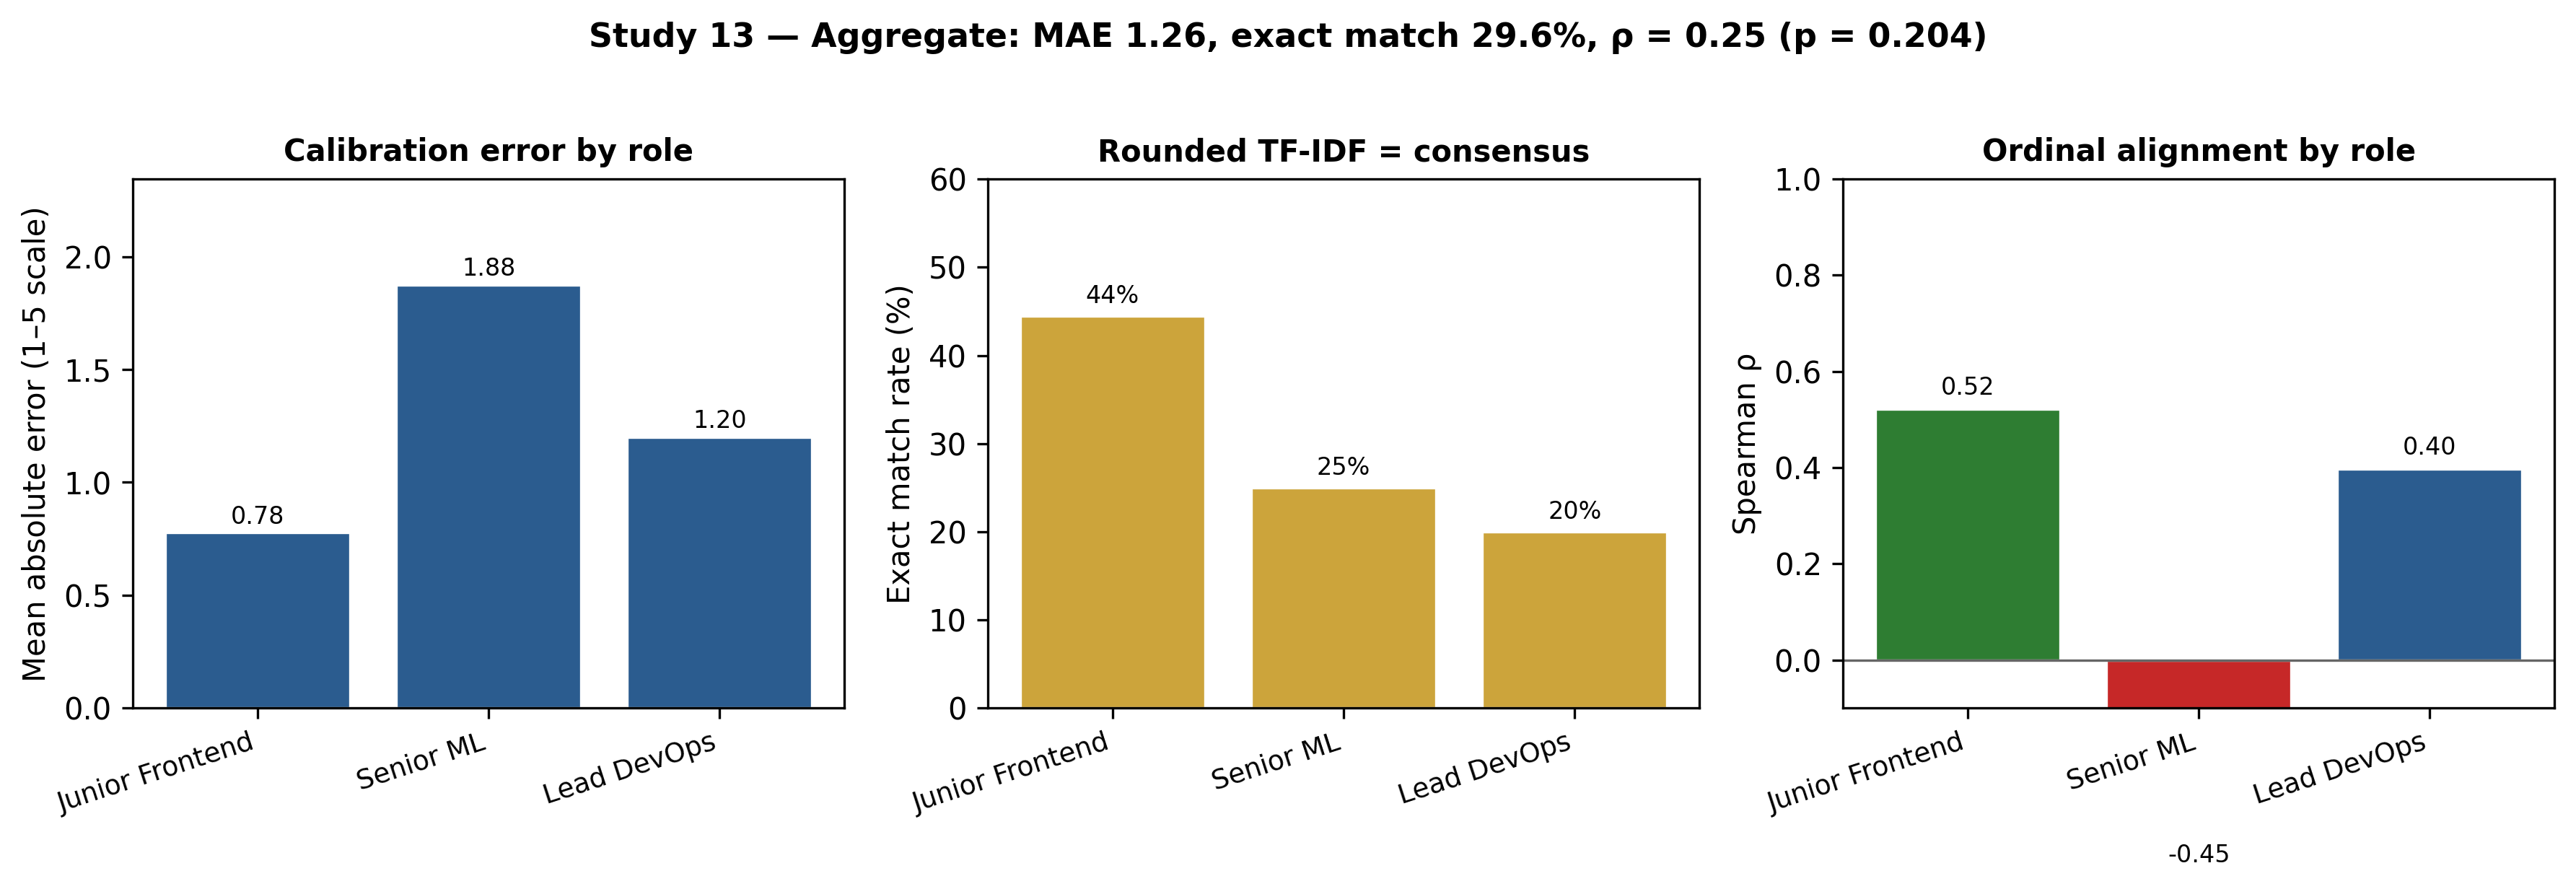
\includegraphics[width=\textwidth]{../evaluation/13-dynamic_tf_idf_recruiter_validation/output/study13_holdout_metrics.png}
    \caption{Study~13: per-hold-out MAE, exact-match rate, and Spearman $\rho$ between consensus priorities and rounded TF-IDF suggestions.}
    \label{fig:study-13-holdout-metrics}
\end{figure}

\begin{figure}[htbp]
    \centering
    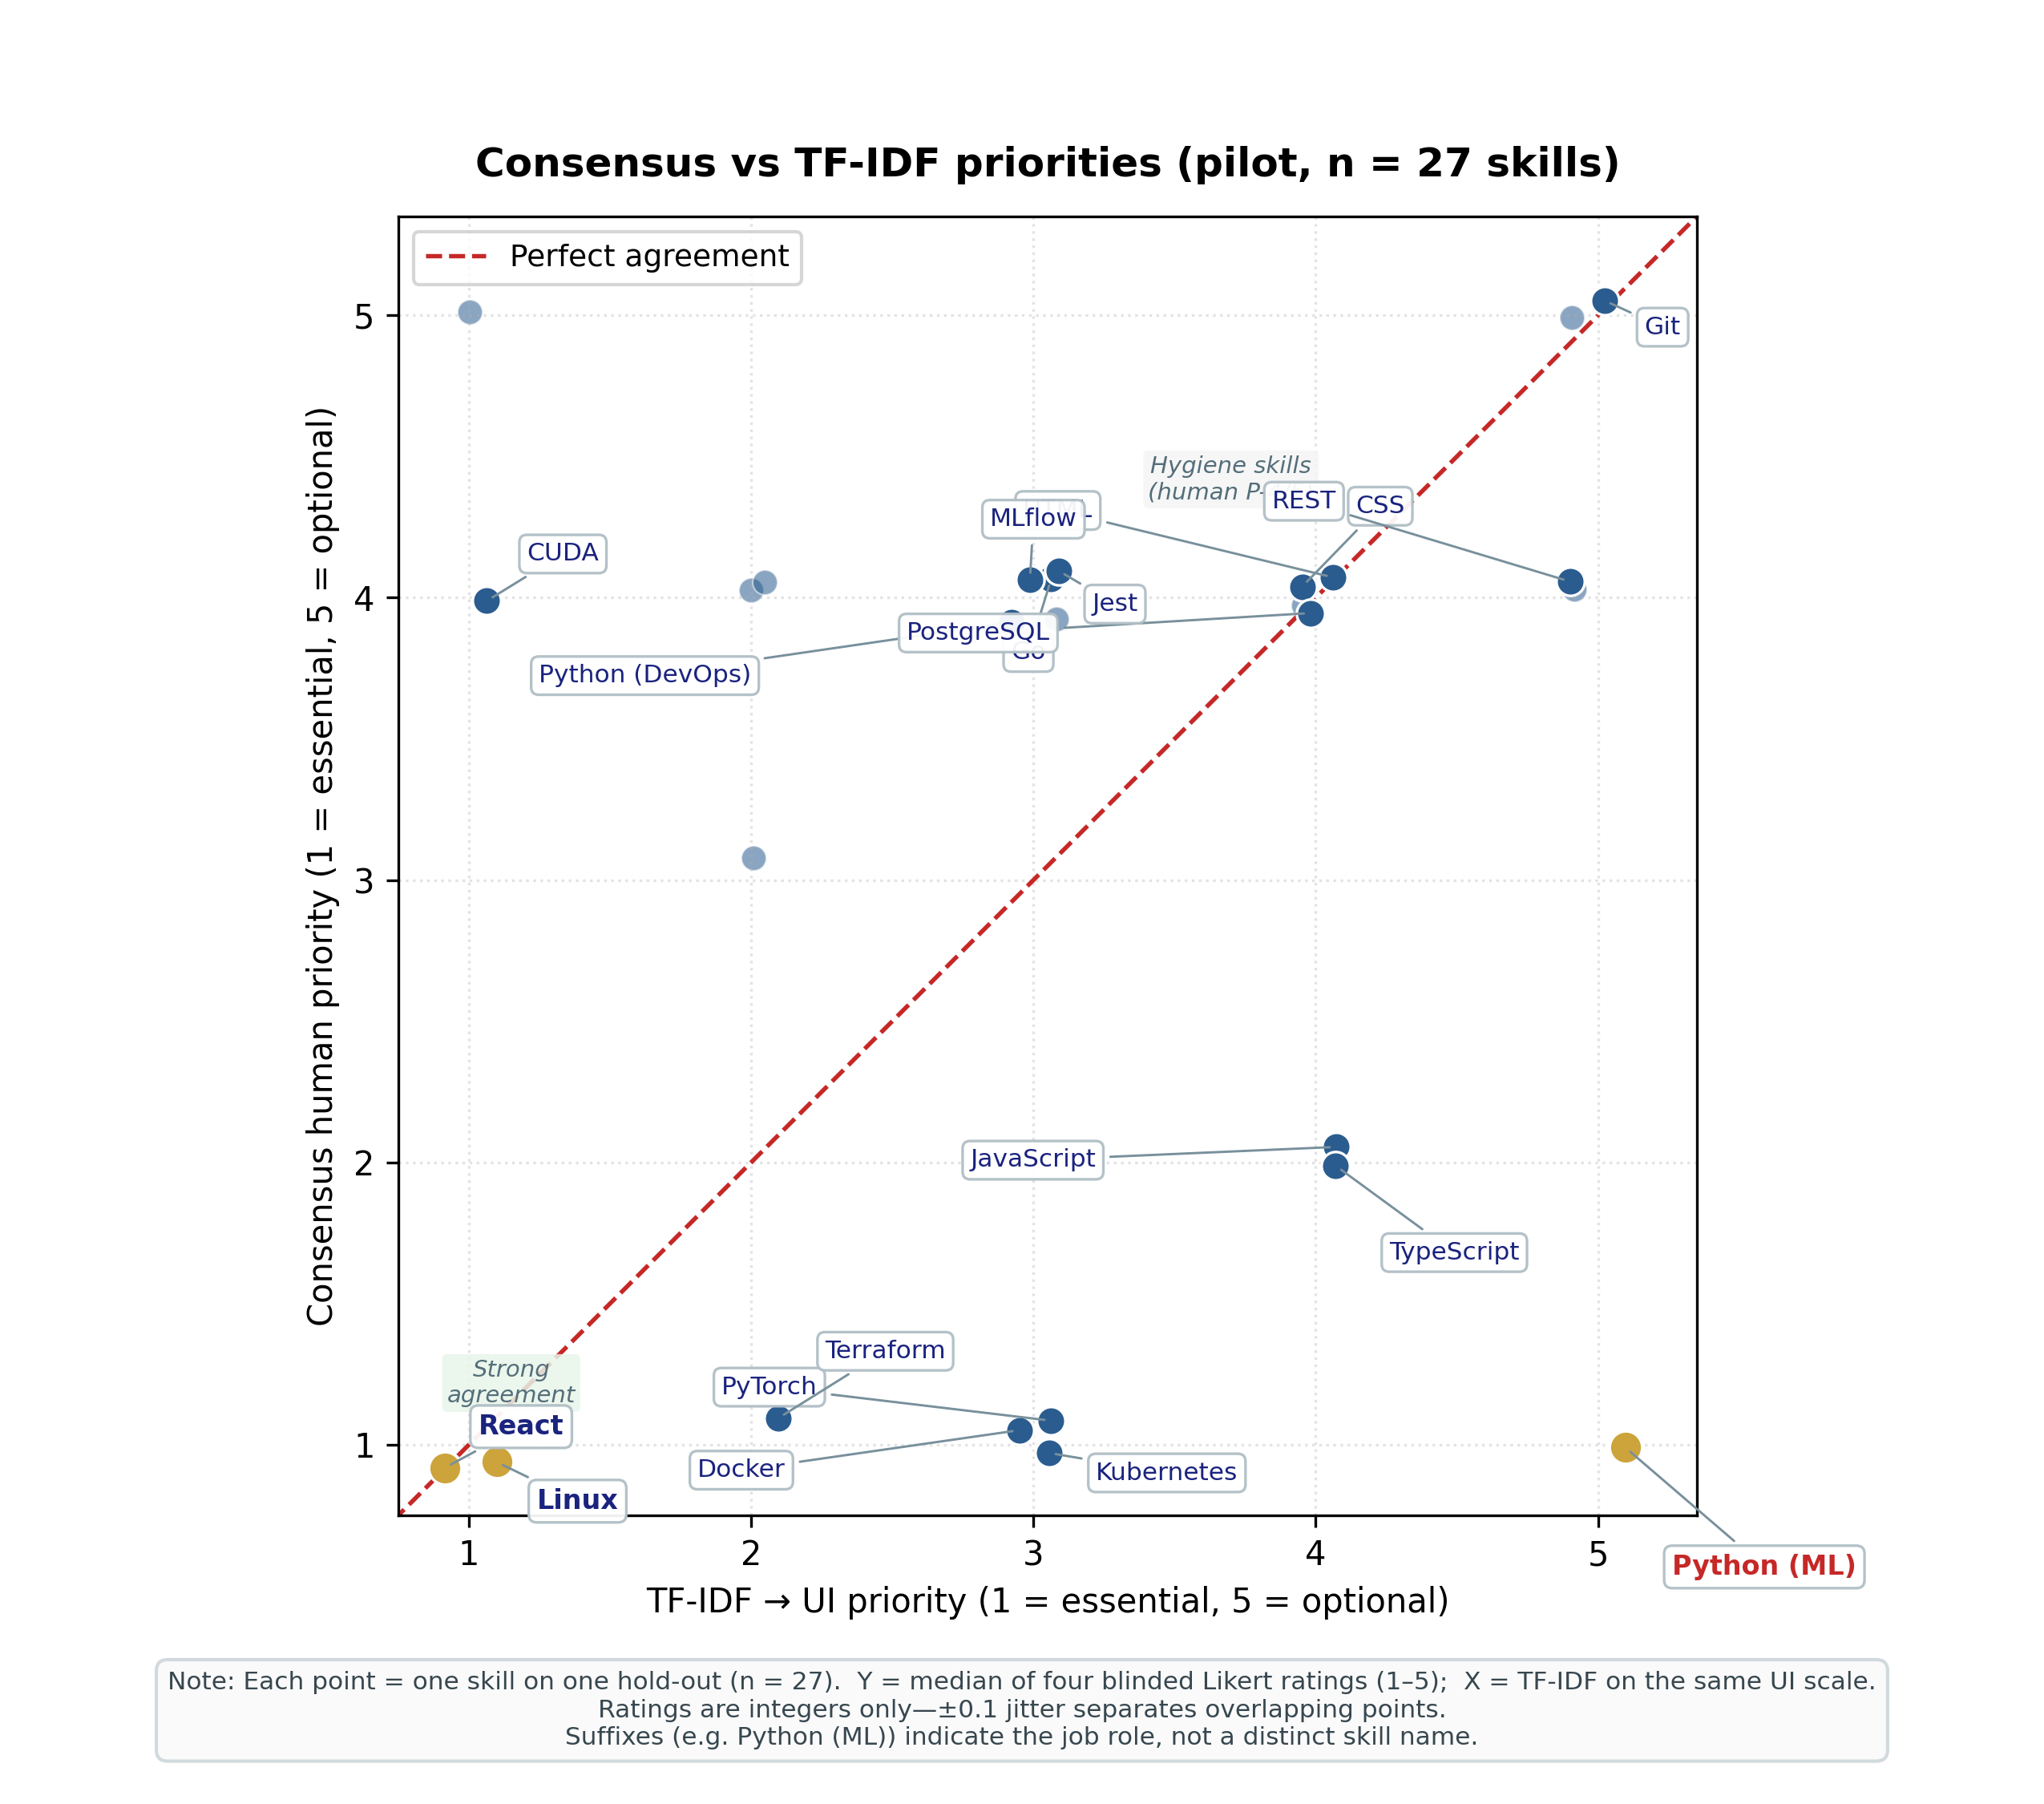
\includegraphics[width=0.72\textwidth]{../evaluation/13-dynamic_tf_idf_recruiter_validation/output/study13_consensus_vs_tfidf_scatter.png}
    \caption{Study~13: consensus human priority vs TF-IDF mapped to UI scale (1 = essential) for 27 skill--role pairs. Points on the diagonal indicate exact agreement; slight positional jitter and footnote on the figure clarify integer-only ratings (see note on chart).}
    \label{fig:study-13-scatter}
\end{figure}

\begin{figure}[htbp]
    \centering
    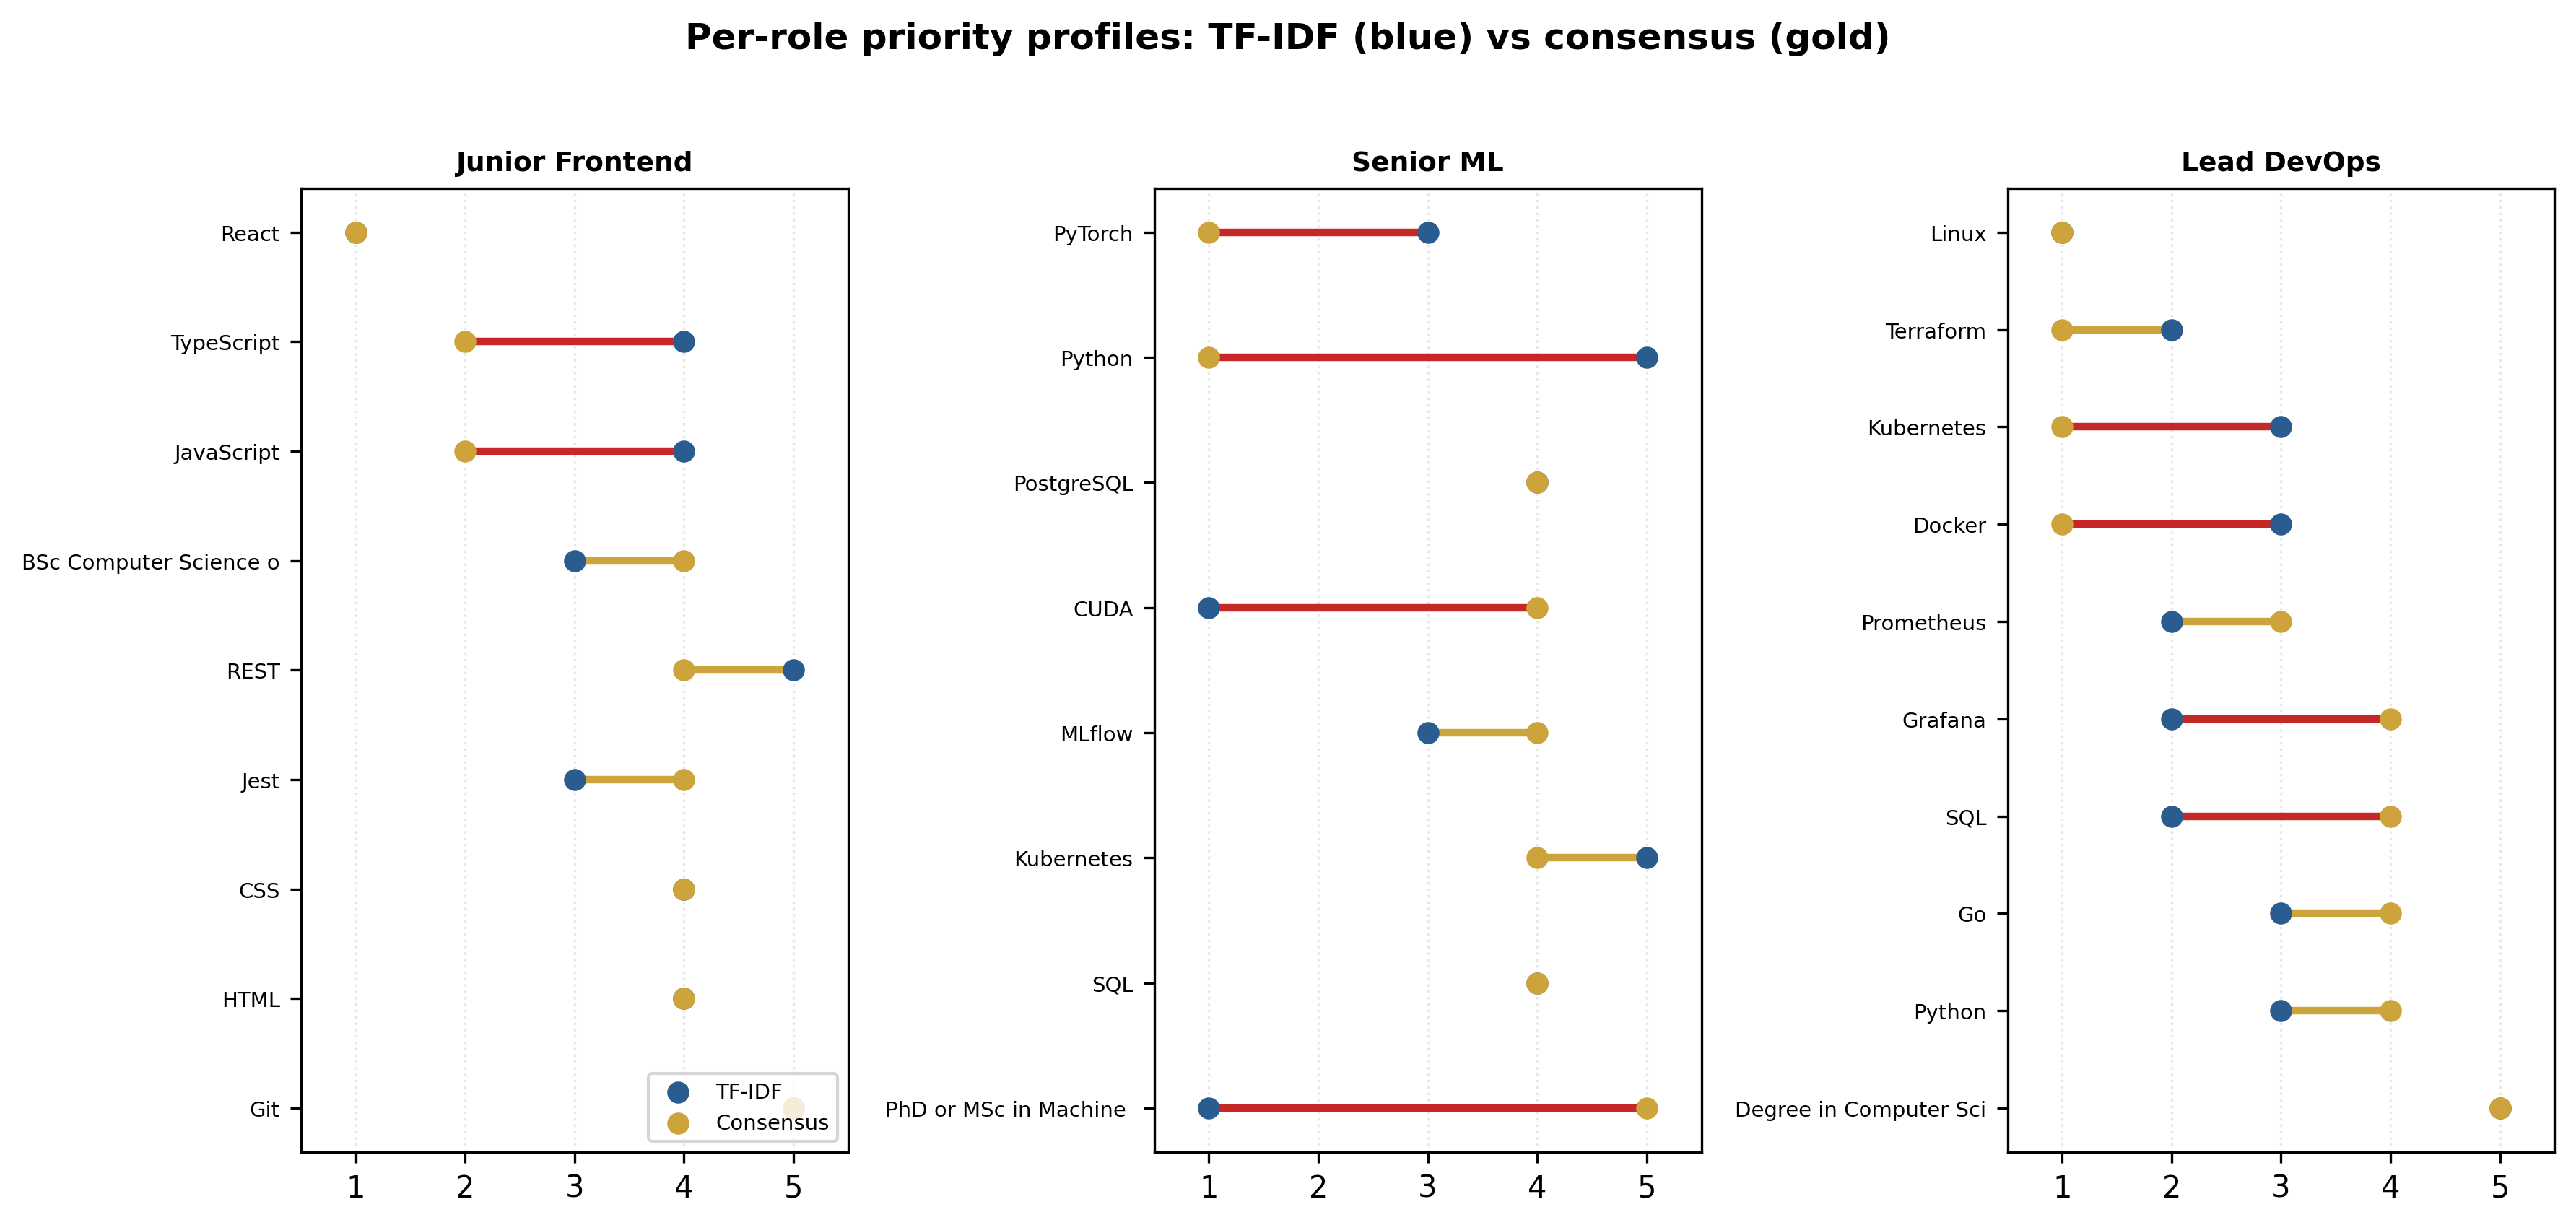
\includegraphics[width=\textwidth]{../evaluation/13-dynamic_tf_idf_recruiter_validation/output/study13_per_role_dumbbell.png}
    \caption{Study~13: per-role dumbbell plots comparing TF-IDF (blue) and consensus (gold) priorities. Green connectors denote exact matches.}
    \label{fig:study-13-dumbbell}
\end{figure}

\begin{figure}[htbp]
    \centering
    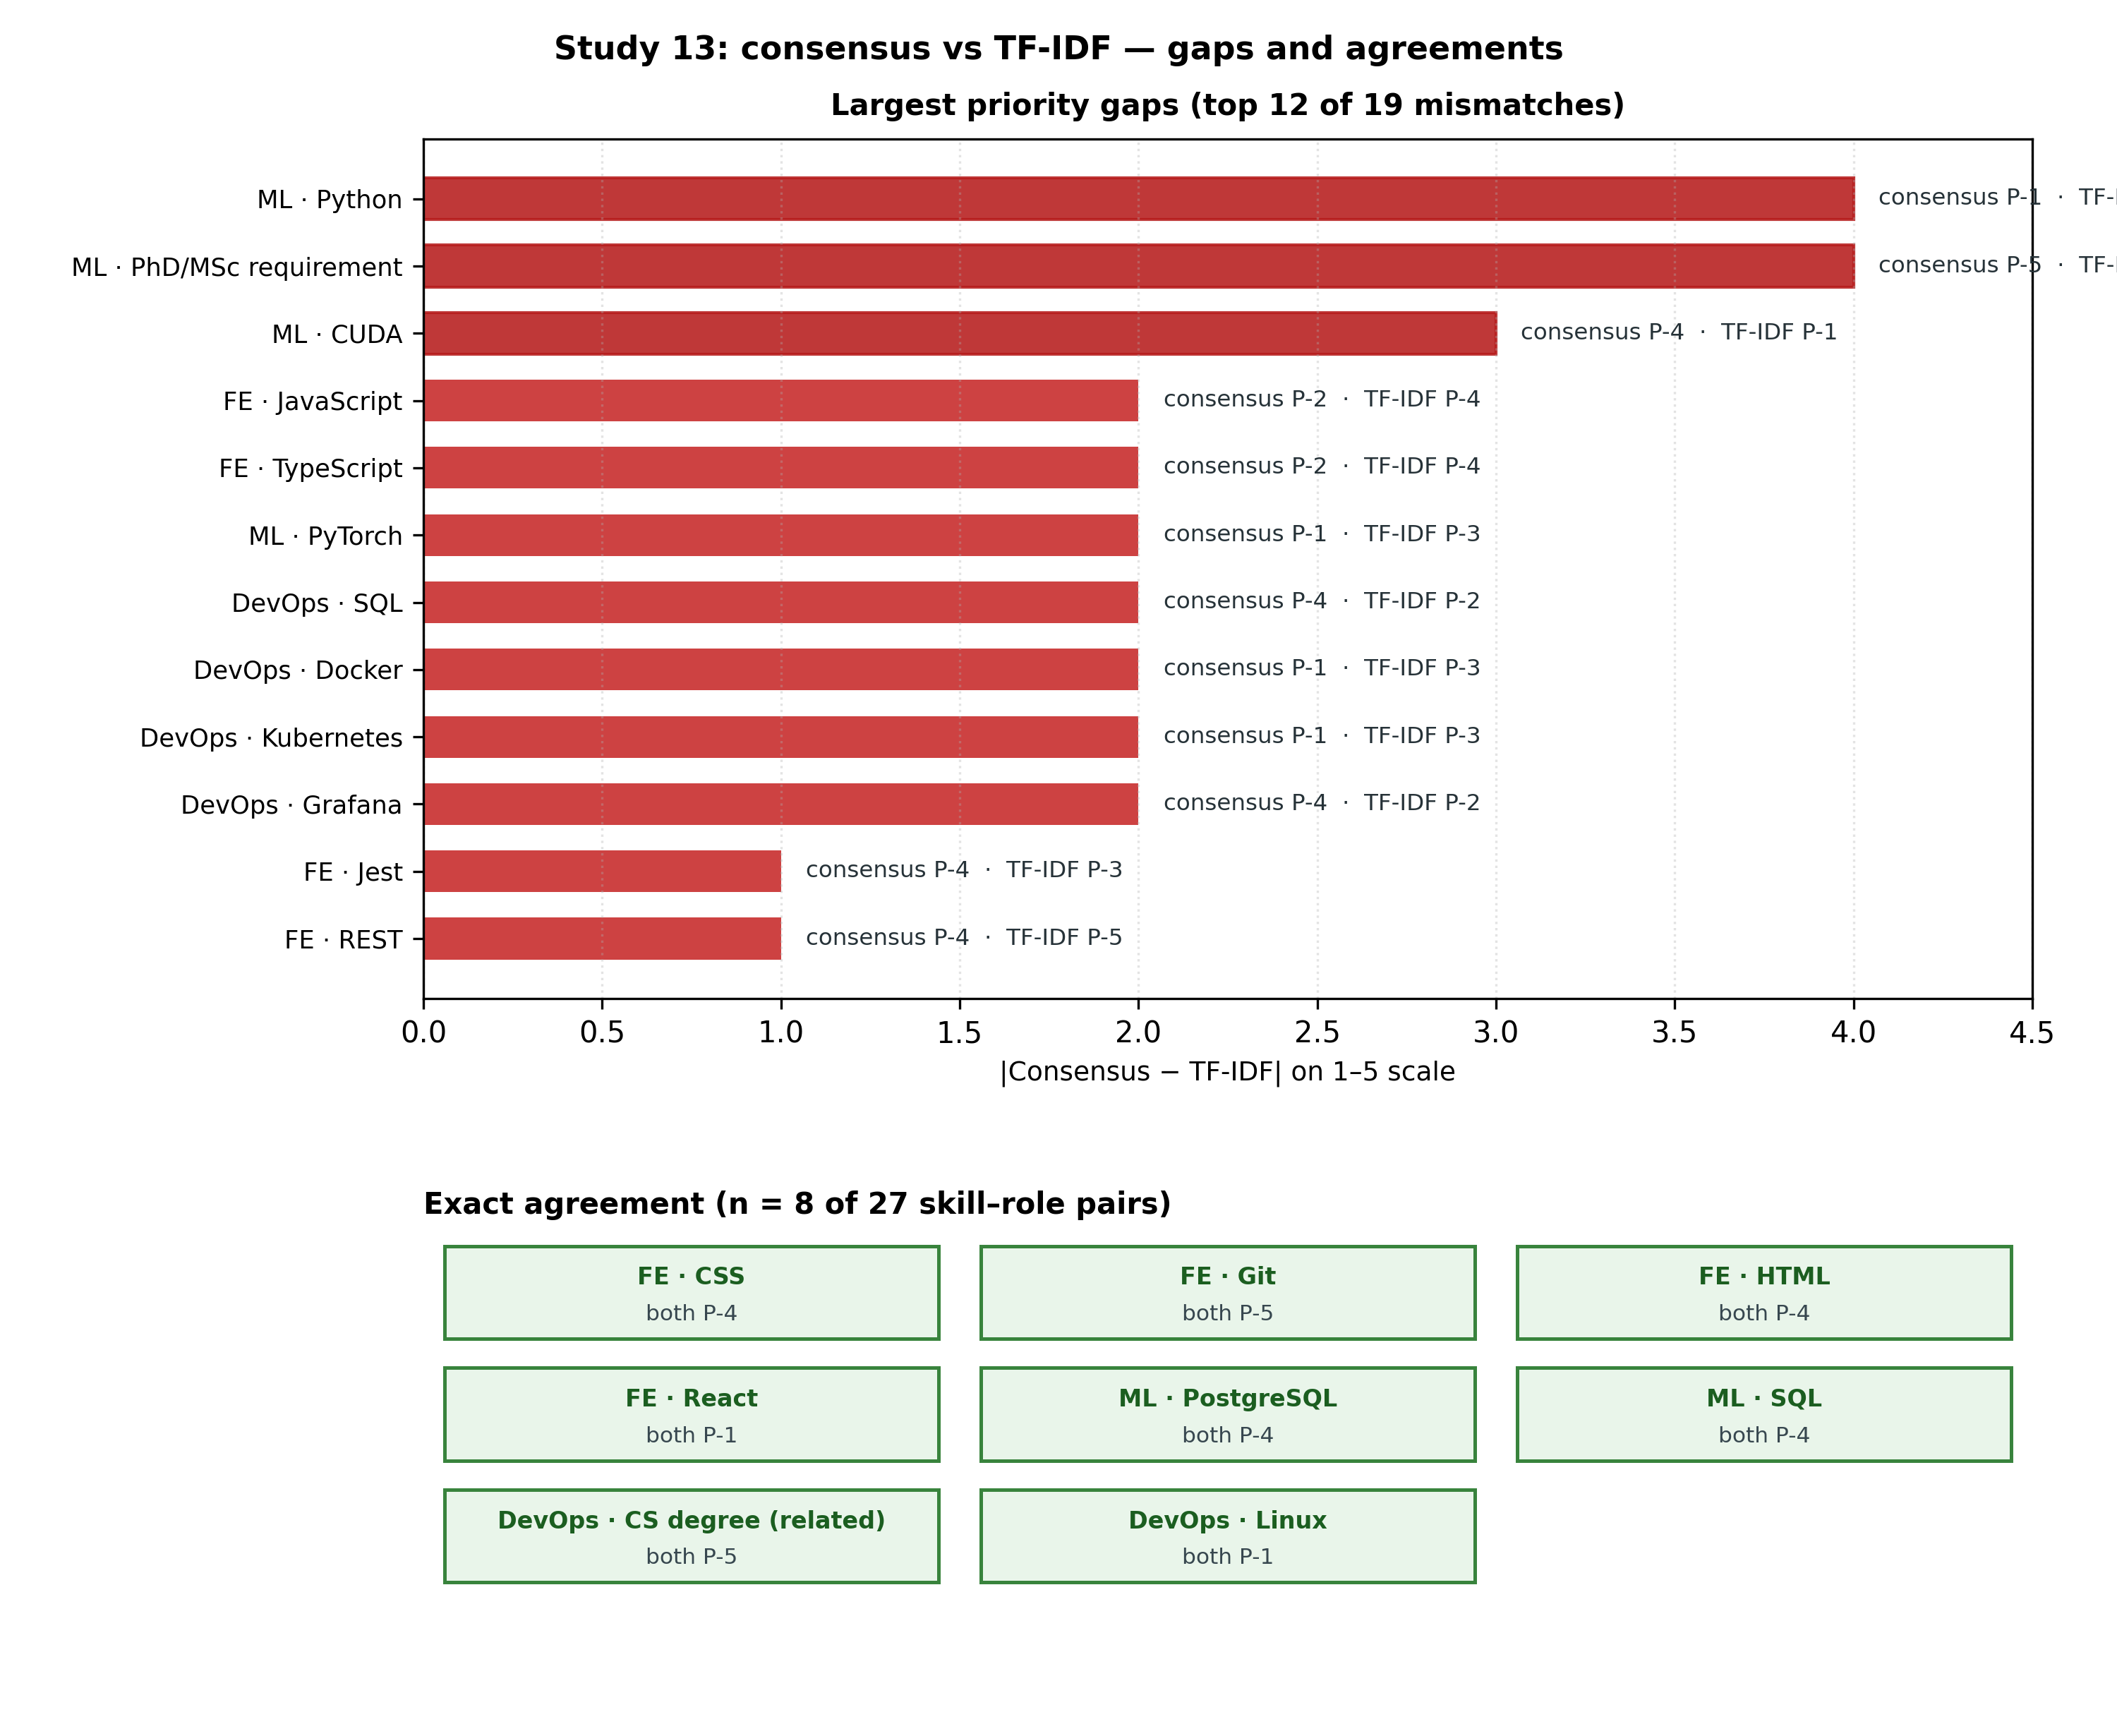
\includegraphics[width=0.92\textwidth]{../evaluation/13-dynamic_tf_idf_recruiter_validation/output/study13_top_misalignments.png}
    \caption{Study~13: largest consensus--TF-IDF gaps (top panel) and eight exact agreements (bottom panel). Axis labels use short chart names (e.g.\ PhD/MSc requirement); full JD strings remain in the evaluation artefacts.}
    \label{fig:study-13-misalignments}
\end{figure}

\begin{figure}[htbp]
    \centering
    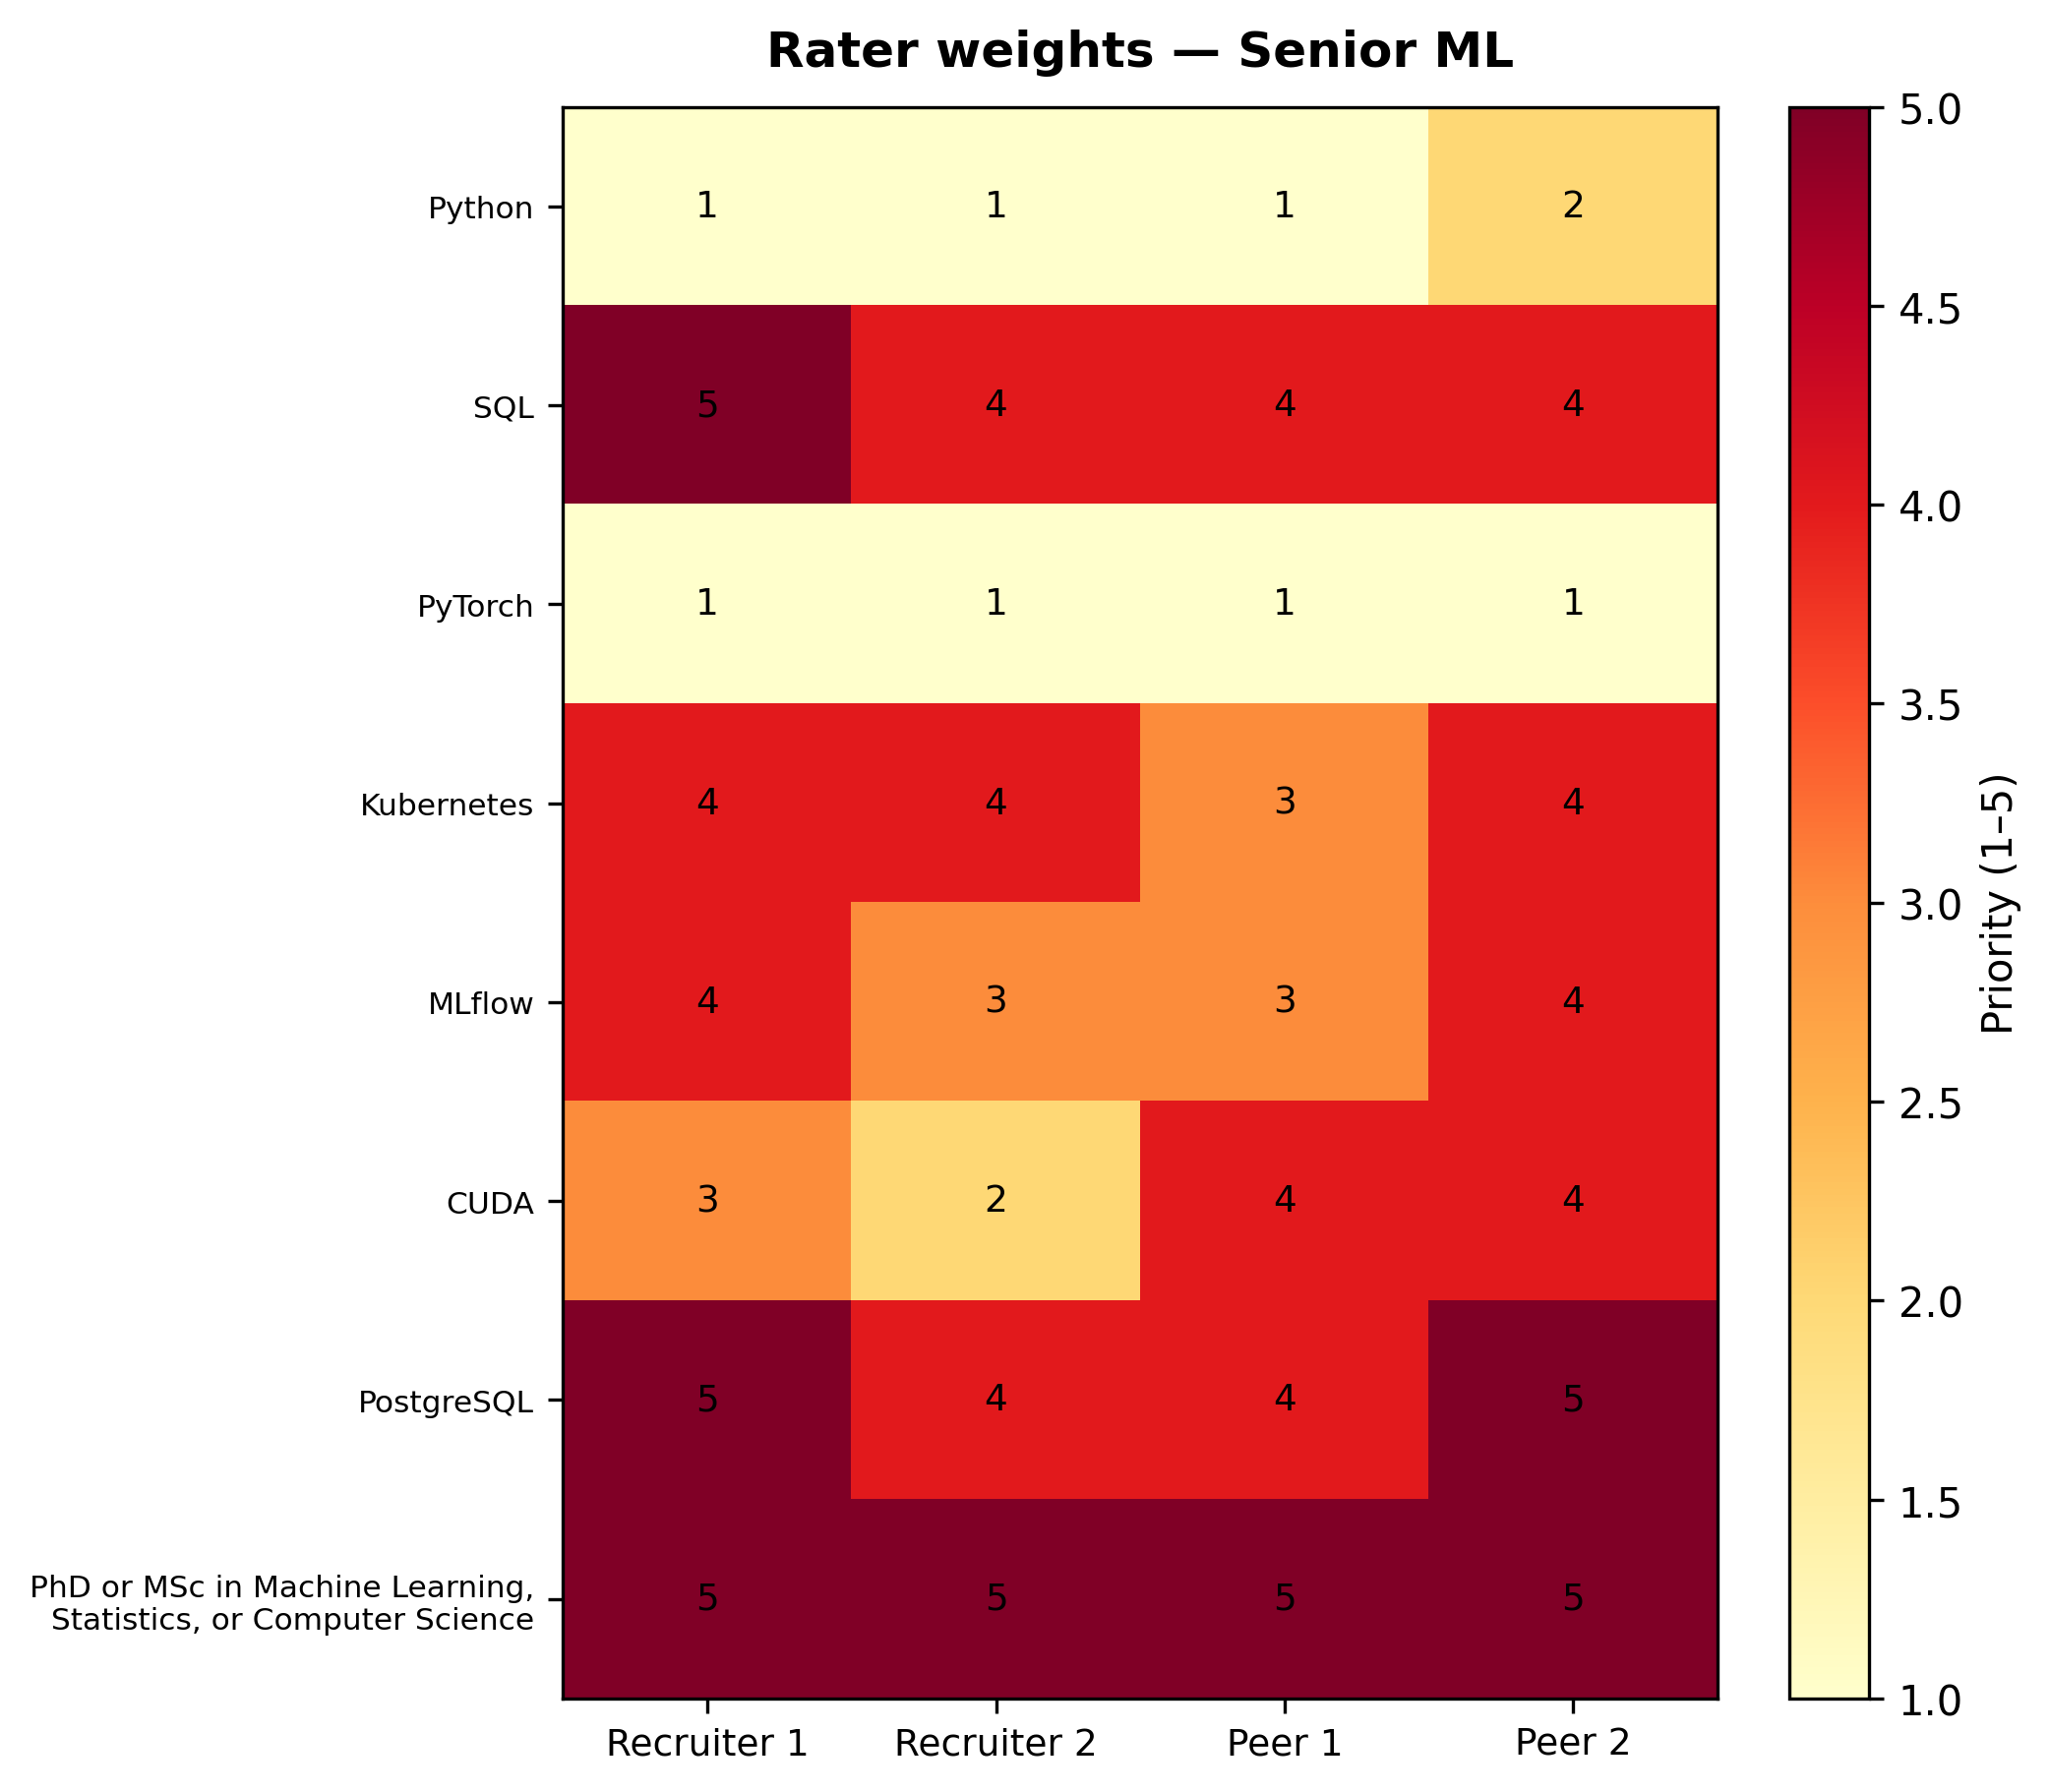
\includegraphics[width=0.88\textwidth]{../evaluation/13-dynamic_tf_idf_recruiter_validation/output/study13_rater_heatmap_ml.png}
    \caption{Study~13: individual rater weights for the senior ML hold-out (per-person 1--5 scores; consensus is the row median). Illustrates headline skills (e.g.\ Python, PyTorch) vs hygiene/degree lines, including unanimous P-5 on the PhD/MSc requirement.}
    \label{fig:study-13-heatmap-ml}
\end{figure}
